\section{test}



\tikzset{every picture/.style={line width=0.75pt}} %set default line width to 0.75pt        

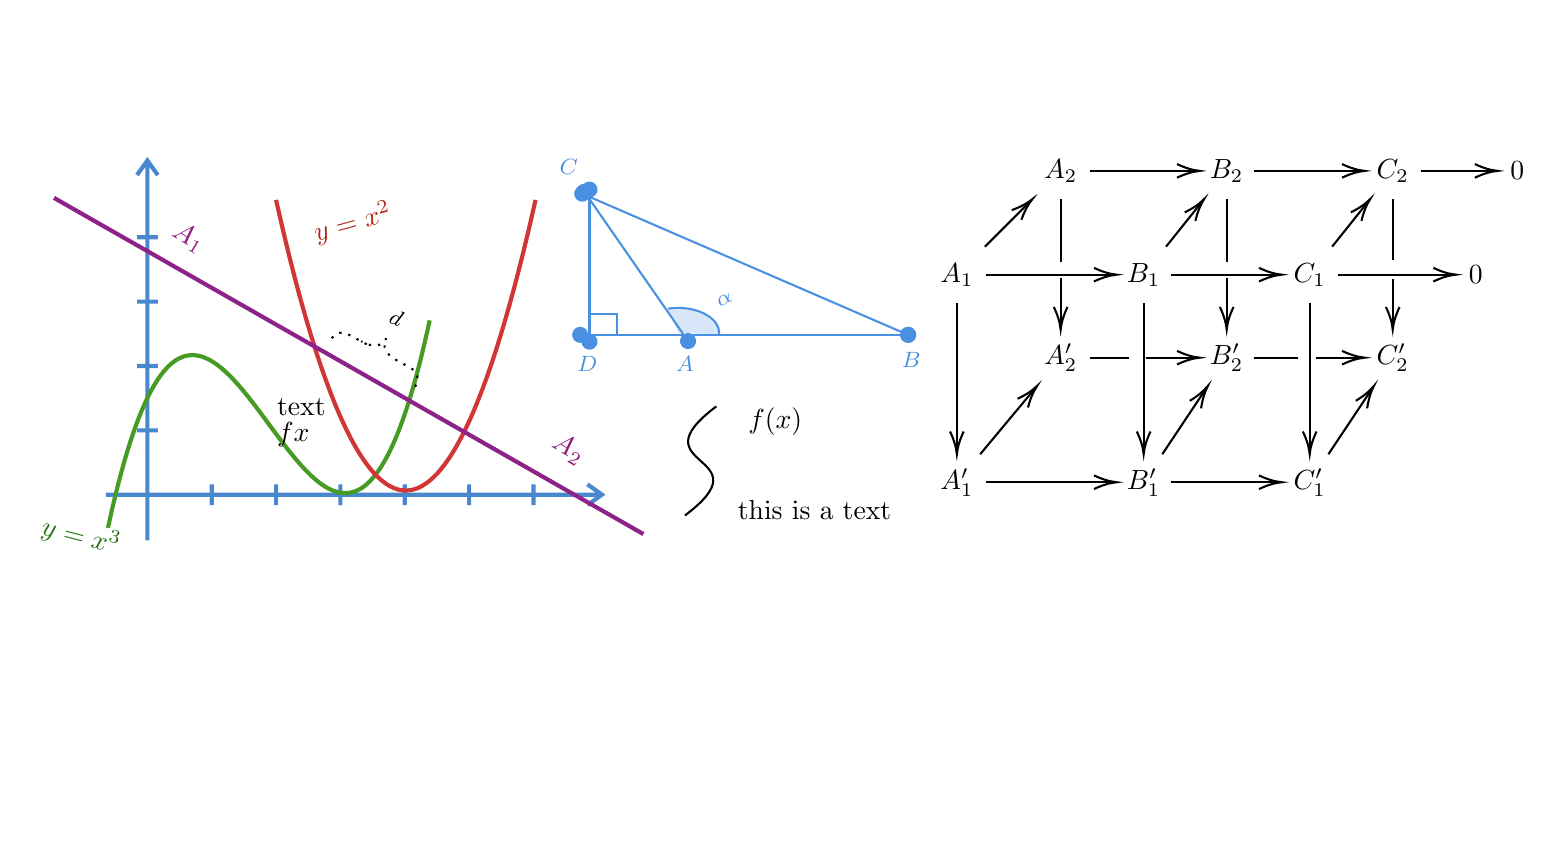
\begin{tikzpicture}[x=0.75pt,y=0.75pt,yscale=-1,xscale=1]
%uncomment if require: \path (0,235); %set diagram left start at 0, and has height of 235

%Straight Lines [id:da9313950171592851] 
\draw [color={rgb, 255:red, 74; green, 144; blue, 226 }  ,draw opacity=1 ]   (274,30) -- (274,103.29) ;
\draw [shift={(274,103.29)}, rotate = 90] [color={rgb, 255:red, 74; green, 144; blue, 226 }  ,draw opacity=1 ][fill={rgb, 255:red, 74; green, 144; blue, 226 }  ,fill opacity=1 ][line width=0.75]      (0, 0) circle [x radius= 3.35, y radius= 3.35]   ;
\draw [shift={(274,30)}, rotate = 90] [color={rgb, 255:red, 74; green, 144; blue, 226 }  ,draw opacity=1 ][fill={rgb, 255:red, 74; green, 144; blue, 226 }  ,fill opacity=1 ][line width=0.75]      (0, 0) circle [x radius= 3.35, y radius= 3.35]   ;
%Straight Lines [id:da0072983473385641595] 
\draw [color={rgb, 255:red, 74; green, 144; blue, 226 }  ,draw opacity=1 ]   (427.58,100) -- (269.5,100) ;
\draw [shift={(269.5,100)}, rotate = 180] [color={rgb, 255:red, 74; green, 144; blue, 226 }  ,draw opacity=1 ][fill={rgb, 255:red, 74; green, 144; blue, 226 }  ,fill opacity=1 ][line width=0.75]      (0, 0) circle [x radius= 3.35, y radius= 3.35]   ;
\draw [shift={(427.58,100)}, rotate = 180] [color={rgb, 255:red, 74; green, 144; blue, 226 }  ,draw opacity=1 ][fill={rgb, 255:red, 74; green, 144; blue, 226 }  ,fill opacity=1 ][line width=0.75]      (0, 0) circle [x radius= 3.35, y radius= 3.35]   ;
%Straight Lines [id:da0611422079179329] 
\draw [color={rgb, 255:red, 74; green, 144; blue, 226 }  ,draw opacity=1 ]   (270.5,32) -- (427.5,100) ;
\draw [shift={(427.5,100)}, rotate = 23.42] [color={rgb, 255:red, 74; green, 144; blue, 226 }  ,draw opacity=1 ][fill={rgb, 255:red, 74; green, 144; blue, 226 }  ,fill opacity=1 ][line width=0.75]      (0, 0) circle [x radius= 3.35, y radius= 3.35]   ;
\draw [shift={(270.5,32)}, rotate = 23.42] [color={rgb, 255:red, 74; green, 144; blue, 226 }  ,draw opacity=1 ][fill={rgb, 255:red, 74; green, 144; blue, 226 }  ,fill opacity=1 ][line width=0.75]      (0, 0) circle [x radius= 3.35, y radius= 3.35]   ;
%Straight Lines [id:da6902289836929021] 
\draw [color={rgb, 255:red, 74; green, 144; blue, 226 }  ,draw opacity=1 ]   (271.5,31) -- (321.5,103) ;
\draw [shift={(321.5,103)}, rotate = 55.22] [color={rgb, 255:red, 74; green, 144; blue, 226 }  ,draw opacity=1 ][fill={rgb, 255:red, 74; green, 144; blue, 226 }  ,fill opacity=1 ][line width=0.75]      (0, 0) circle [x radius= 3.35, y radius= 3.35]   ;
\draw [shift={(271.5,31)}, rotate = 55.22] [color={rgb, 255:red, 74; green, 144; blue, 226 }  ,draw opacity=1 ][fill={rgb, 255:red, 74; green, 144; blue, 226 }  ,fill opacity=1 ][line width=0.75]      (0, 0) circle [x radius= 3.35, y radius= 3.35]   ;
%Shape: Arc [id:dp012460516914444497] 
\draw  [draw opacity=0][fill={rgb, 255:red, 74; green, 144; blue, 226 }  ,fill opacity=0.22 ] (311.81,87.37) .. controls (313.42,87.12) and (315.12,86.99) .. (316.87,87) .. controls (327.75,87.07) and (336.54,92.5) .. (336.5,99.12) .. controls (336.5,99.34) and (336.49,99.56) .. (336.47,99.78) -- (316.8,99) -- cycle ; \draw  [color={rgb, 255:red, 74; green, 144; blue, 226 }  ,draw opacity=1 ] (311.81,87.37) .. controls (313.42,87.12) and (315.12,86.99) .. (316.87,87) .. controls (327.75,87.07) and (336.54,92.5) .. (336.5,99.12) .. controls (336.5,99.34) and (336.49,99.56) .. (336.47,99.78) ;
%Straight Lines [id:da012774030553635018] 
\draw [color={rgb, 255:red, 74; green, 144; blue, 226 }  ,draw opacity=1 ]   (274,90) -- (287.04,90) -- (287.04,100.78) ;
%Shape: Axis 2D [id:dp048941842347560494] 
\draw [color={rgb, 255:red, 73; green, 135; blue, 206 }  ,draw opacity=1 ][line width=1.5]  (41,177) -- (280,177)(61,16) -- (61,199) (273,172) -- (280,177) -- (273,182) (56,23) -- (61,16) -- (66,23) (92,172) -- (92,182)(123,172) -- (123,182)(154,172) -- (154,182)(185,172) -- (185,182)(216,172) -- (216,182)(247,172) -- (247,182)(56,146) -- (66,146)(56,115) -- (66,115)(56,84) -- (66,84)(56,53) -- (66,53) ;
\draw   ;
%Shape: Polynomial [id:dp29246577559714826] 
\draw  [color={rgb, 255:red, 70; green, 155; blue, 36 }  ,draw opacity=1 ][line width=1.5]  (42,193) .. controls (93.67,-47) and (145.33,333) .. (197,93) ;
%Shape: Parabola [id:dp636758281566334] 
\draw  [color={rgb, 255:red, 209; green, 53; blue, 53 }  ,draw opacity=1 ][line width=1.5]  (123,35) .. controls (164.67,221.67) and (206.33,221.67) .. (248,35) ;
%Straight Lines [id:da5751643928734858] 
\draw [color={rgb, 255:red, 141; green, 34; blue, 137 }  ,draw opacity=1 ][line width=1.5]    (16,34) -- (300,196) ;
%Shape: Brace [id:dp8862990797251067] 
\draw  [dash pattern={on 0.84pt off 2.51pt}] (190,125) .. controls (192.21,120.89) and (191.25,117.73) .. (187.14,115.52) -- (181.62,112.56) .. controls (175.75,109.41) and (173.91,105.77) .. (176.12,101.66) .. controls (173.91,105.77) and (169.87,106.25) .. (164,103.1)(166.64,104.52) -- (158.48,100.14) .. controls (154.37,97.93) and (151.21,98.89) .. (149,103) ;
%Curve Lines [id:da4259284507066625] 
\draw    (320,187) .. controls (360,157) and (295.13,164.46) .. (335.13,134.46) ;

% Text Node
\draw (339,83) node  [font=\footnotesize,color={rgb, 255:red, 74; green, 144; blue, 226 }  ,opacity=1 ,rotate=-333.43]  {$\alpha $};
% Text Node
\draw (264,19) node  [font=\footnotesize,color={rgb, 255:red, 74; green, 144; blue, 226 }  ,opacity=1 ]  {$C$};
% Text Node
\draw (273,114) node  [font=\footnotesize,color={rgb, 255:red, 74; green, 144; blue, 226 }  ,opacity=1 ]  {$D$};
% Text Node
\draw (320,114) node  [font=\footnotesize,color={rgb, 255:red, 74; green, 144; blue, 226 }  ,opacity=1 ]  {$A$};
% Text Node
\draw (429,112) node  [font=\footnotesize,color={rgb, 255:red, 74; green, 144; blue, 226 }  ,opacity=1 ]  {$B$};
% Text Node
\draw (451,71) node    {$A_{1}$};
% Text Node
\draw (501,21) node    {$A_{2}$};
% Text Node
\draw (451,171) node    {$A'_{1}$};
% Text Node
\draw (581,21) node    {$B_{2}$};
% Text Node
\draw (661,21) node    {$C_{2}$};
% Text Node
\draw (541,71) node    {$B_{1}$};
% Text Node
\draw (621,71) node    {$C_{1}$};
% Text Node
\draw (501,111) node    {$A'_{2}$};
% Text Node
\draw (581,111) node    {$B'_{2}$};
% Text Node
\draw (661,111) node    {$C'_{2}$};
% Text Node
\draw (541,171) node    {$B'_{1}$};
% Text Node
\draw (621,171) node    {$C'_{1}$};
% Text Node
\draw (721,21) node    {$0$};
% Text Node
\draw (701,71) node    {$0$};
% Text Node
\draw (81,53) node  [color={rgb, 255:red, 146; green, 29; blue, 130 }  ,opacity=1 ,rotate=-30.96]  {$A_{1}$};
% Text Node
\draw (264,155) node  [color={rgb, 255:red, 145; green, 25; blue, 123 }  ,opacity=1 ,rotate=-30.96]  {$A_{2}$};
% Text Node
\draw (29,197) node  [color={rgb, 255:red, 36; green, 114; blue, 18 }  ,opacity=1 ,rotate=-14.47]  {$y=x^{3}$};
% Text Node
\draw (160,46) node  [color={rgb, 255:red, 179; green, 35; blue, 24 }  ,opacity=1 ,rotate=-344.74]  {$y=x^{2}$};
% Text Node
\draw (181,92) node  [font=\footnotesize,rotate=-22.93]  {$d$};
% Text Node
\draw (122,129) node [anchor=north west][inner sep=0.75pt]   [align=left] {text};
% Text Node
\draw (122,140.4) node [anchor=north west][inner sep=0.75pt]    {$fx$};
% Text Node
\draw (344,178) node [anchor=north west][inner sep=0.75pt]   [align=left] {this is a text};
% Text Node
\draw (349,133.4) node [anchor=north west][inner sep=0.75pt]    {$f( x)$};
% Connection
\draw    (515,21) -- (566,21) ;
\draw [shift={(568,21)}, rotate = 180] [color={rgb, 255:red, 0; green, 0; blue, 0 }  ][line width=0.75]    (10.93,-3.29) .. controls (6.95,-1.4) and (3.31,-0.3) .. (0,0) .. controls (3.31,0.3) and (6.95,1.4) .. (10.93,3.29)   ;
% Connection
\draw    (594,21) -- (645.5,21) ;
\draw [shift={(647.5,21)}, rotate = 180] [color={rgb, 255:red, 0; green, 0; blue, 0 }  ][line width=0.75]    (10.93,-3.29) .. controls (6.95,-1.4) and (3.31,-0.3) .. (0,0) .. controls (3.31,0.3) and (6.95,1.4) .. (10.93,3.29)   ;
% Connection
\draw    (464.5,57.5) -- (486.09,35.91) ;
\draw [shift={(487.5,34.5)}, rotate = 495] [color={rgb, 255:red, 0; green, 0; blue, 0 }  ][line width=0.75]    (10.93,-3.29) .. controls (6.95,-1.4) and (3.31,-0.3) .. (0,0) .. controls (3.31,0.3) and (6.95,1.4) .. (10.93,3.29)   ;
% Connection
\draw    (465,71) -- (526,71) ;
\draw [shift={(528,71)}, rotate = 180] [color={rgb, 255:red, 0; green, 0; blue, 0 }  ][line width=0.75]    (10.93,-3.29) .. controls (6.95,-1.4) and (3.31,-0.3) .. (0,0) .. controls (3.31,0.3) and (6.95,1.4) .. (10.93,3.29)   ;
% Connection
\draw    (554,71) -- (605.5,71) ;
\draw [shift={(607.5,71)}, rotate = 180] [color={rgb, 255:red, 0; green, 0; blue, 0 }  ][line width=0.75]    (10.93,-3.29) .. controls (6.95,-1.4) and (3.31,-0.3) .. (0,0) .. controls (3.31,0.3) and (6.95,1.4) .. (10.93,3.29)   ;
% Connection
\draw    (551.8,57.5) -- (568.95,36.06) ;
\draw [shift={(570.2,34.5)}, rotate = 488.66] [color={rgb, 255:red, 0; green, 0; blue, 0 }  ][line width=0.75]    (10.93,-3.29) .. controls (6.95,-1.4) and (3.31,-0.3) .. (0,0) .. controls (3.31,0.3) and (6.95,1.4) .. (10.93,3.29)   ;
% Connection
\draw    (631.8,57.5) -- (648.95,36.06) ;
\draw [shift={(650.2,34.5)}, rotate = 488.66] [color={rgb, 255:red, 0; green, 0; blue, 0 }  ][line width=0.75]    (10.93,-3.29) .. controls (6.95,-1.4) and (3.31,-0.3) .. (0,0) .. controls (3.31,0.3) and (6.95,1.4) .. (10.93,3.29)   ;
% Connection
\draw    (451,84.5) -- (451,155.5) ;
\draw [shift={(451,157.5)}, rotate = 270] [color={rgb, 255:red, 0; green, 0; blue, 0 }  ][line width=0.75]    (10.93,-3.29) .. controls (6.95,-1.4) and (3.31,-0.3) .. (0,0) .. controls (3.31,0.3) and (6.95,1.4) .. (10.93,3.29)   ;
% Connection
\draw    (465,171) -- (526,171) ;
\draw [shift={(528,171)}, rotate = 180] [color={rgb, 255:red, 0; green, 0; blue, 0 }  ][line width=0.75]    (10.93,-3.29) .. controls (6.95,-1.4) and (3.31,-0.3) .. (0,0) .. controls (3.31,0.3) and (6.95,1.4) .. (10.93,3.29)   ;
% Connection
\draw    (554,171) -- (605.5,171) ;
\draw [shift={(607.5,171)}, rotate = 180] [color={rgb, 255:red, 0; green, 0; blue, 0 }  ][line width=0.75]    (10.93,-3.29) .. controls (6.95,-1.4) and (3.31,-0.3) .. (0,0) .. controls (3.31,0.3) and (6.95,1.4) .. (10.93,3.29)   ;
% Connection
\draw    (630,157.5) -- (650.89,126.16) ;
\draw [shift={(652,124.5)}, rotate = 483.69] [color={rgb, 255:red, 0; green, 0; blue, 0 }  ][line width=0.75]    (10.93,-3.29) .. controls (6.95,-1.4) and (3.31,-0.3) .. (0,0) .. controls (3.31,0.3) and (6.95,1.4) .. (10.93,3.29)   ;
% Connection
\draw    (550,157.5) -- (570.89,126.16) ;
\draw [shift={(572,124.5)}, rotate = 483.69] [color={rgb, 255:red, 0; green, 0; blue, 0 }  ][line width=0.75]    (10.93,-3.29) .. controls (6.95,-1.4) and (3.31,-0.3) .. (0,0) .. controls (3.31,0.3) and (6.95,1.4) .. (10.93,3.29)   ;
% Connection
\draw    (462.25,157.5) -- (488.47,126.04) ;
\draw [shift={(489.75,124.5)}, rotate = 489.81] [color={rgb, 255:red, 0; green, 0; blue, 0 }  ][line width=0.75]    (10.93,-3.29) .. controls (6.95,-1.4) and (3.31,-0.3) .. (0,0) .. controls (3.31,0.3) and (6.95,1.4) .. (10.93,3.29)   ;
% Connection
\draw    (515,111) -- (533.95,111)(541.95,111) -- (566,111) ;
\draw [shift={(568,111)}, rotate = 180] [color={rgb, 255:red, 0; green, 0; blue, 0 }  ][line width=0.75]    (10.93,-3.29) .. controls (6.95,-1.4) and (3.31,-0.3) .. (0,0) .. controls (3.31,0.3) and (6.95,1.4) .. (10.93,3.29)   ;
% Connection
\draw    (594,111) -- (615.25,111)(624.25,111) -- (645.5,111) ;
\draw [shift={(647.5,111)}, rotate = 180] [color={rgb, 255:red, 0; green, 0; blue, 0 }  ][line width=0.75]    (10.93,-3.29) .. controls (6.95,-1.4) and (3.31,-0.3) .. (0,0) .. controls (3.31,0.3) and (6.95,1.4) .. (10.93,3.29)   ;
% Connection
\draw    (501,34.5) -- (501,64.66)(501,72.66) -- (501,95.5) ;
\draw [shift={(501,97.5)}, rotate = 270] [color={rgb, 255:red, 0; green, 0; blue, 0 }  ][line width=0.75]    (10.93,-3.29) .. controls (6.95,-1.4) and (3.31,-0.3) .. (0,0) .. controls (3.31,0.3) and (6.95,1.4) .. (10.93,3.29)   ;
% Connection
\draw    (581,34.5) -- (581,64.66)(581,72.66) -- (581,95.5) ;
\draw [shift={(581,97.5)}, rotate = 270] [color={rgb, 255:red, 0; green, 0; blue, 0 }  ][line width=0.75]    (10.93,-3.29) .. controls (6.95,-1.4) and (3.31,-0.3) .. (0,0) .. controls (3.31,0.3) and (6.95,1.4) .. (10.93,3.29)   ;
% Connection
\draw    (661,34.5) -- (661,64.16)(661,73.16) -- (661,95.5) ;
\draw [shift={(661,97.5)}, rotate = 270] [color={rgb, 255:red, 0; green, 0; blue, 0 }  ][line width=0.75]    (10.93,-3.29) .. controls (6.95,-1.4) and (3.31,-0.3) .. (0,0) .. controls (3.31,0.3) and (6.95,1.4) .. (10.93,3.29)   ;
% Connection
\draw    (541,84.5) -- (541,155.5) ;
\draw [shift={(541,157.5)}, rotate = 270] [color={rgb, 255:red, 0; green, 0; blue, 0 }  ][line width=0.75]    (10.93,-3.29) .. controls (6.95,-1.4) and (3.31,-0.3) .. (0,0) .. controls (3.31,0.3) and (6.95,1.4) .. (10.93,3.29)   ;
% Connection
\draw    (621,84.5) -- (621,155.5) ;
\draw [shift={(621,157.5)}, rotate = 270] [color={rgb, 255:red, 0; green, 0; blue, 0 }  ][line width=0.75]    (10.93,-3.29) .. controls (6.95,-1.4) and (3.31,-0.3) .. (0,0) .. controls (3.31,0.3) and (6.95,1.4) .. (10.93,3.29)   ;
% Connection
\draw    (674.5,21) -- (709.5,21) ;
\draw [shift={(711.5,21)}, rotate = 180] [color={rgb, 255:red, 0; green, 0; blue, 0 }  ][line width=0.75]    (10.93,-3.29) .. controls (6.95,-1.4) and (3.31,-0.3) .. (0,0) .. controls (3.31,0.3) and (6.95,1.4) .. (10.93,3.29)   ;
% Connection
\draw    (634.5,71) -- (689.5,71) ;
\draw [shift={(691.5,71)}, rotate = 180] [color={rgb, 255:red, 0; green, 0; blue, 0 }  ][line width=0.75]    (10.93,-3.29) .. controls (6.95,-1.4) and (3.31,-0.3) .. (0,0) .. controls (3.31,0.3) and (6.95,1.4) .. (10.93,3.29)   ;

\end{tikzpicture}



\section{随机变量的引入}

在实际问题中,随机试验的结果可以用数量来表示,由此就产生了随机变量的概念.

有些试验结果本身与数值有关(本身就是一个数);在有些试验中,试验结果看来与数值无关,但我们可以引进一个变量来表示它的各种结果.也就是说,把试验结果数值化.这种对应关系在数学上理解为定义了一种实值单值函数

\section{随机变量的特点}

它随试验结果的不同而取不同的值,因而在试验之前只知道它可能取值的范围,而不能预先肯定它将取哪个值.

由于试验结果的出现具有一定的概率,于是这种实值函数取每个值和每个确定范围内的值也有一定的概率, 所以称这种定义在样本空间 $S$ 上的实值单值函数 $X= X(e)$为随机变量

\section{优势}

\begin{enumerate}
    \item 引入随机变量后,对随机现象统计规律的研究,就由对事件及事件概率的研究扩大为对随机变量及其取值规律的研究
    \item 易于表示
    \item 和原来集合的表示等价
\end{enumerate}

\section{常见随机变量}

\subsection{离散型随机变量}

公式法

$$
\boldsymbol{P}\left\{\boldsymbol{X}=\boldsymbol{x}_{k}\right\}=\boldsymbol{p}_{k}, \boldsymbol{k}=1,2, \cdots
$$

列表法
  
$$X \sim\left(\begin{array}{lllll}x_{1} & x_{2} & \cdots & x_{n} & \cdots \\ p_{1} & p_{2} & \cdots & p_{n} & \cdots\end{array}\right)$$

\begin{center}
    \begin{tabular}{|c|c|c|c|c|}
    \hline $ \boldsymbol{X} $ & $ \boldsymbol{x}_{1} $ & $ \boldsymbol{x}_{2} $ & $ \cdots $ & $ \boldsymbol{x}_{n} \cdots $ \\
    \hline $ \boldsymbol{p}_{k} $ & $ \boldsymbol{p}_{1} $ & $ \boldsymbol{p}_{2} $ & $ \cdots $ & $ \boldsymbol{p}_{n} \cdots $ \\
    \hline
    \end{tabular}
\end{center}


\subsection{两点分布}

特殊的二项分布(n = 1)
\begin{center}
   \begin{tabular}{|c|c|c|}
    \hline $ \mathrm{X} $ & $0$ & $1 $\\
    \hline$ p_{k} $ & $ 1-\mathrm{p} $ & $ \mathrm{p} $ \\
    \hline
    \end{tabular}

\subsection{(n 重)伯努利试验, 二项分布} 
\end{center}


$$
P\{X=k\}=\left(\begin{array}{l}
n \\
k
\end{array}\right) p^{k}(1-p)^{n-k} \quad k=0,1, \cdots, n
$$

$$
\begin{array}{c|cccccc}
\boldsymbol{X} & \mathbf{0} & \mathbf{1} & \cdots & \boldsymbol{k} & \cdots & \boldsymbol{n} \\
\hline \boldsymbol{p}_{\boldsymbol{k}} & \boldsymbol{q}^{n} & \left(\begin{array}{l}
\boldsymbol{n} \\
\mathbf{1}
\end{array}\right) \boldsymbol{p q}^{n-1} & \cdots & \left(\begin{array}{l}
\boldsymbol{n} \\
\boldsymbol{k}
\end{array}\right) \boldsymbol{p}^{k} \boldsymbol{q}^{n-k} & \cdots & \boldsymbol{p}^{n}
\end{array}
$$

\subsubsection{二项分布性质}

\begin{itemize}
    \item 将伯努利试验 $E$独立地重复地进行 $n$ 次 ,则称这一串重复的独立试验为 $n$ 重伯努利试验.伯努利试验对试验结果没有等可能的要求 “重复”是指这 $n$ 次试验中 $P(A)= p$ 保持不变.“独立”是指各次试验的结果互不影响.
    \item 每次试验条件相同
    \item 每次试验只考虑两个互逆结果 $A$ 或 $\overline{A}$
    \item 各次试验相互独立
    \item 二项分布描述的是 $n$ 重伯努利试验中事件 $A$ 出现的次数 $X$ 的分布律
\end{itemize}

\subsubsection{二项分布单峰性质}

若在$k_0$处,概率 P{X=k}达到最大(称$k_0$为随机变量 X 的最可能值)

$$
\left\{\begin{array}{l}
\frac{P\left\{X=k_{0}\right\}}{P\left\{X=k_{0}+1\right\}} \geq 1 \\
\frac{P\left\{X=k_{0}\right\}}{P\left\{X=k_{0}-1\right\}} \geq 1
\end{array}\right.
$$

得
$$ (n+1) p-1 \leq k\_{0} \leq(n+1) p $$

$$
k_{0}=\left\{\begin{array}{ll}
(n+1) p \text { 和 }(n+1) p-1, & \text { 当 }(\boldsymbol{n}+\mathbf{1}) \boldsymbol{p} \text { 为整数 }, \\
{[(n+1) p],} & \text { 其它 },
\end{array}\right.
$$

\subsection{泊松分布}

$$
\boldsymbol{P}\{\boldsymbol{X}=\boldsymbol{k}\}=\frac{\lambda^{k} \mathrm{e}^{-\lambda}}{\boldsymbol{k} !}, \quad \boldsymbol{k}=\mathbf{0}, \mathbf{1}, \mathbf{2}, \cdots
$$

其中$\lambda > 0$是常数, 则称 X 服从参数为$\lambda$的泊松分布, 记作
$$ X \sim \pi(\lambda) $$


\begin{theorem}[泊松定理]
    \label{thm:Poission}
泊松分布是作为二项分布的近似,于 1837 年由法国数学家泊松引入的.
$$
\lim _{n \rightarrow \infty} C_{n}^{k} p_{n}^{k}\left(1-p_{n}\right)^{n-k}=e^{-\lambda} \frac{\lambda^{k}}{k !}\quad (\lambda = np)
$$
\end{theorem}

\subsection{连续型随机变量}

\subsection{均匀分布}

$$
f(x)=\left\{\begin{array}{cc}
\frac{1}{b-a}, & a<x<b \\
0, & \text { 其它 }
\end{array}\right.
$$

$$ X \sim U(a,b) $$

$$
F(x)=P\{X \leq x\}=\left\{\begin{array}{ll}
0, & x<a \\
\frac{x-a}{b-a}, & a \leq x<b \\
1 & x \geq b
\end{array}\right.
$$

\subsection{指数分布}

$$
f(x)=\left\{\begin{array}{ll}
\frac{1}{\theta} e^{-x / \theta}, & x>0 \\
0, & \text { 其它, }
\end{array}\right.
$$

$$
F(x)=P\{X \leq x\}=\left\{\begin{array}{ll}
1-e^{-x / \theta}, & x>0 \\
0, & \text { 其它 }
\end{array}\right.
$$

\subsection{正态分布}

$$
f(x)=\frac{1}{\sqrt{2 \pi} \sigma} e^{-\frac{(x-\mu)^{2}}{2 \sigma^{2}}}, \quad-\infty<x<\infty
$$

\subsection{标准正态分布}

$$
\text { 若 } X \sim N\left(\mu, \sigma^{2}\right), \text { 则 } Z=\frac{X-\mu}{\sigma} \sim N(\mathbf{0}, 1)
$$

\section{随机变量的分布函数}

\section{随机变量的分布函数性质}

对任意实数 $x_1<x_2$,随机点落在区间$( x_1 ,  x_2 ]$内的概率为:

$$
P\{ x_1<X  \le  x_2\} =P\{ X  \le   x_2 \} - P\{ X  \le   x_1 \}= F(x_2)-F(x_1)
$$

$$
\begin{array}{l}
F(-\infty)=\lim_{x \rightarrow-\infty} F(x)=0 \\
F(+\infty)=\lim_{x \rightarrow+\infty} F(x)=1
\end{array}
$$

\section{连续型随机变量及其概率密度}

$$ f(x) \geq 0 $$

$$ \int\_{-\infty}^{\infty} f(x) d x=1 $$

% todo: 边缘分布、条件分布

\section{随机变量的数字特征}

\subsection{方差}


$$
 D(X) = E \Big\{ [x-E(X)] \Big\}
$$

$$
 D(X) = E(X^2) - [E(X)] ^2
$$

\subsubsection{方差性质}

$$
 D(C) = 0
$$

$$
 D(CX) = C^2D(X)
$$

$$
 D(X+C) = D(X)
$$

X 和 Y 相互独立时,

$$
 D(X+Y) = D(X)+D(Y)
$$

D(X) = 0 等价于 $
 P[X = E(X)] = 1
$

\begin{theorem}[切比雪夫不等式]
    \label{Chebyshev\'sInequality}
$$
\begin{aligned}
    P(|X-\mu| \ge \varepsilon) \le \frac{\sigma^2}{\varepsilon^2}
\end{aligned}
$$

$$
 P(|X-\mu| < \varepsilon) \ge 1 - \frac{\sigma^2}{\varepsilon^2}
$$
\end{theorem}

\subsection{协方差}

$$
 Cov(X,Y) = E\Big\{ [X - E(X)][Y-E(Y)] \Big\}
$$

$$
 Cov(X,Y) = E(XY) - E(X)E(Y)
$$

\subsubsection{协方差性质}

$$
 D(X+Y) = D(X)+D(Y)+2Cov(X,Y)
$$

$$
 Cov(X,Y) = Cov(Y,X)
$$

$$
 Cov(X,X) = D(X)
$$

$$ Cov(X,c) = 0 $$

$$ Cov(a X + b, Y) = a Cov( X,Y) $$

$$ Cov(aX, bY) = ab Cov(X, Y) $$

$$ Cov(X_1 + X_2 , Y) = Cov(X_1 , Y) + Cov(X_2 , Y) $$

对于随机变量序列 $ X_{1}, \ldots, X_{n} $ 与 $ Y_{1}, \ldots, Y_{m} $, 有
$$
\operatorname{cov}\left(\sum_{i=1}^{n} X_{i}, \sum_{j=1}^{m} Y_{j}\right)=\sum_{i=1}^{n} \sum_{j=1}^{m} \operatorname{cov}\left(X_{i}, Y_{j}\right)
$$

对于随机变量序列 $ X_{1}, \ldots, X_{n} $, 有

$$
\operatorname{var}\left(\sum_{i=1}^{n} X_{i}\right)=\sum_{i=1}^{n} \operatorname{var}\left(X_{i}\right)+2 \sum_{i, j: i<j} \operatorname{cov}\left(X_{i}, X_{j}\right)
$$

\subsection{相关系数}

$$
 \rho_{XY} =   \frac{Cov(X,Y) }{\sqrt{D(X)} \sqrt{D(Y)}}
$$

相关系数是刻划两个变量间线性相关程度的一个重要的数字特征. 相关系数也可以看成协方差:一种剔除了两个变量量纲影响、标准化后的特殊协方差。

\subsection{X, Y 不相关时候的性质}

若 $\rho_{X Y}=0$, 称 X 和 Y 不(线性)相关。

\begin{corollary}
    独立一定是不相关,不相关不一定独立。
\end{corollary}

\begin{theorem}
    若随机变量 $X$ 与 Y 的方差都存在,且均不为零; 则下列四个命题等价。
    \begin{enumerate}
        \item $\rho_{X Y}=0$
        \item $\operatorname{Cov}(X, Y)=0$
        \item $E(X Y)=E (X) E (Y)$
        \item $D(X \pm Y)=D X+D Y_{\circ}$
    \end{enumerate}
\end{theorem}